% begin module inverse-function-graph
\begin{frame}
\begin{tabular}{cc}
\ \only<handout:0| -4>{%
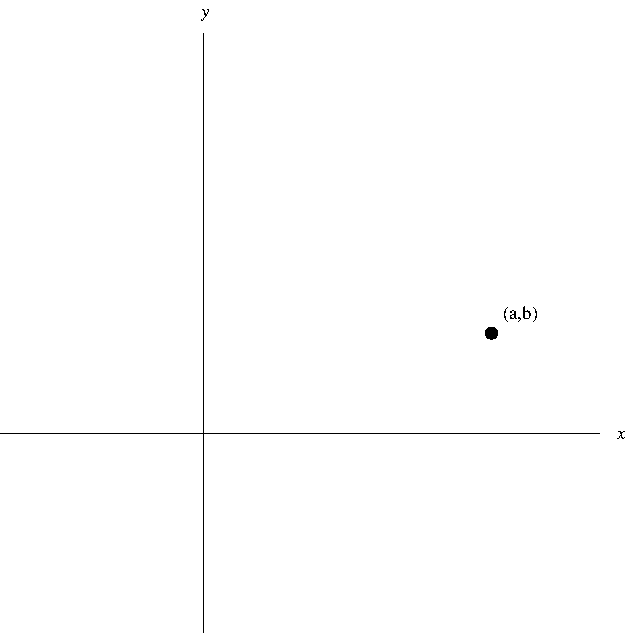
\includegraphics[height=4cm]{inverse-functions/pictures/07-01-reflecta.pdf}%
}%
\only<handout:0| 5>{%
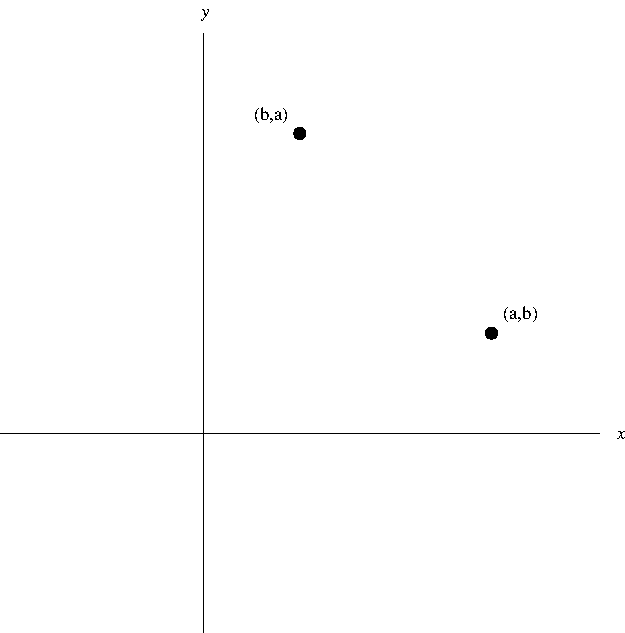
\includegraphics[height=4cm]{inverse-functions/pictures/07-01-reflectb.pdf}%
}%
\only<handout:1| 6->{%
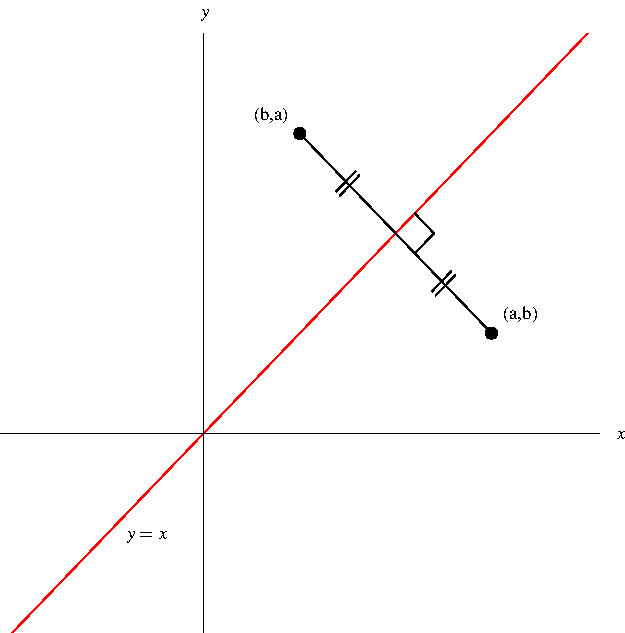
\includegraphics[height=4cm]{inverse-functions/pictures/07-01-reflectc.pdf}%
}%
&%
\only<handout:0| -6>{%
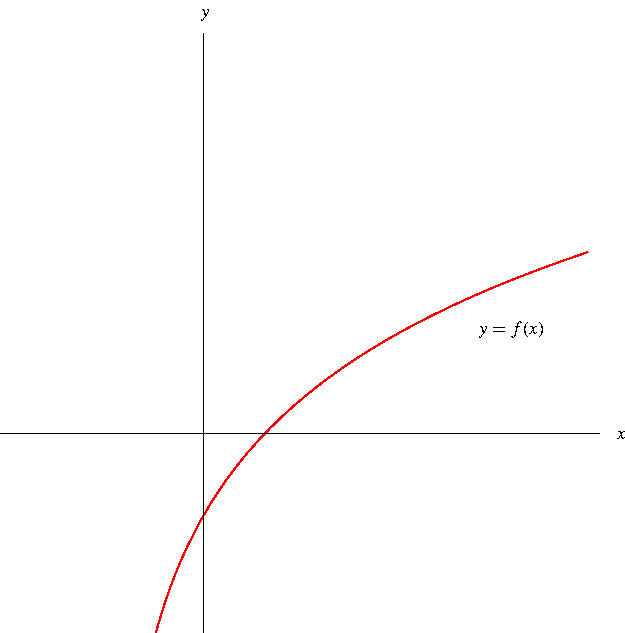
\includegraphics[height=4cm]{inverse-functions/pictures/07-01-reflect-functionb.pdf}%
}%
\only<handout:1| 7->{%
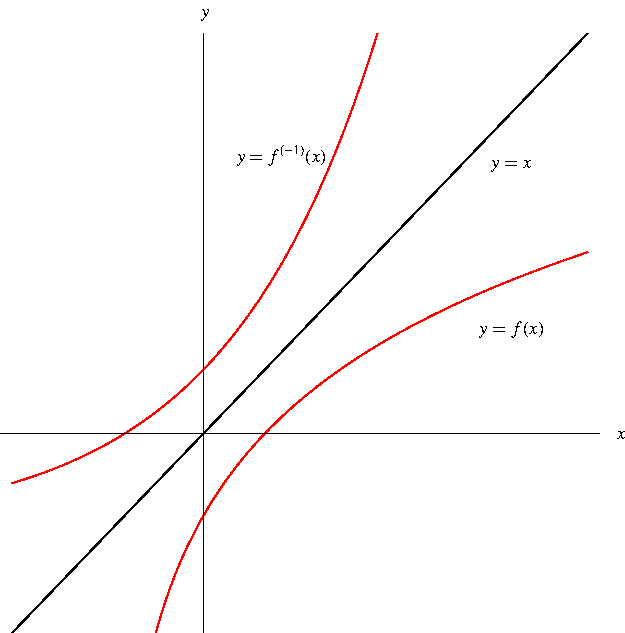
\includegraphics[height=4cm]{inverse-functions/pictures/07-01-reflect-functiona.pdf}%
}%
\end{tabular}

The principle of switching $x$ and $y$ suggests a way to derive the graph of $f^{-1}$ from that of $f$:
\begin{itemize}
\item<2->  Suppose $(a,b)$ is on the graph of $f$.
\item<3->  Then $f(a) = b$.
\item<4->  Then $f^{-1}(b) = a$.
\item<5->  Then $(b,a)$ is on the graph of $f^{-1}$.
\item<6->  $(b,a)$ is the reflection of $(a,b)$ in the line $y = x$.
\item<7->  Therefore the graph of $f^{-1}$ is obtained by reflecting the graph of $f$ in the line $y = x$.
\end{itemize}
\end{frame}
% end module inverse-function-graph
